\subsubsection{Balansowanie rozmiarów obszarów}
Ten etap algorytmu wywoływany jest zawsze po procedurze optymalizacji długości granic.
Odpowiedzialny jest za wyrównaniu wielkości pól, które nie są idealnie równe po
wywołaniu algorytmu LAM.
Przez autorów artykułu \cite{1364754} został opisany, jako algorytm zachłanny, natomiast nie było
podanych więcej szczegółów na jego temat.

W związku z powyższym zaimplementowałem poniższe rozwiązanie.
Algorytm również korzysta z mechanizmu do budowania zbiorów helpful i balancing, to jest z obliczania wartości
helpfulness dla wierzchołków.
Zachłannie wybierane są wierzchołki z największą wartością helpfulness, dopóki pola obszarów nie zostaną
zbalansowane do oczekiwanej wartości różnicy pól.
Obszary balansują się zabierając wierzchołki obszarów sąsiednich.
Oznacza to, że jeśli wywoływany jest algorytm optymalizacji granic między obszarami $A$ oraz $B$, gdzie obszar $A$
jest większy od obszaru $B$, to po wyrównaniu granicy pomiędzy nimi obszar $A$ odda część wierzchołków obszarowi $B$.

\vspace{4mm}
\begin{figure}[h]
\begin{subfigure}{.5\textwidth}
    \centering
    \fbox{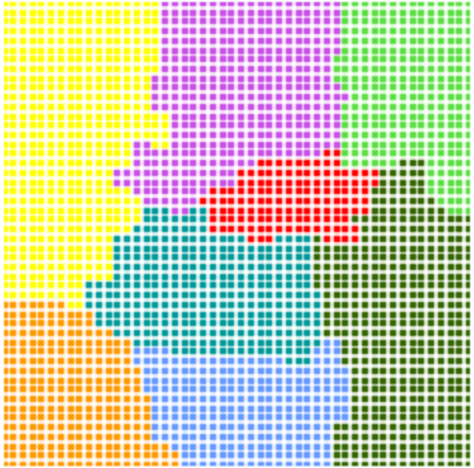
\includegraphics[width=\imgss\textwidth]{images/fields-balacing/1}}
    \caption[short]{krok 1}
\end{subfigure}
\begin{subfigure}{.5\textwidth}
    \centering
    \fbox{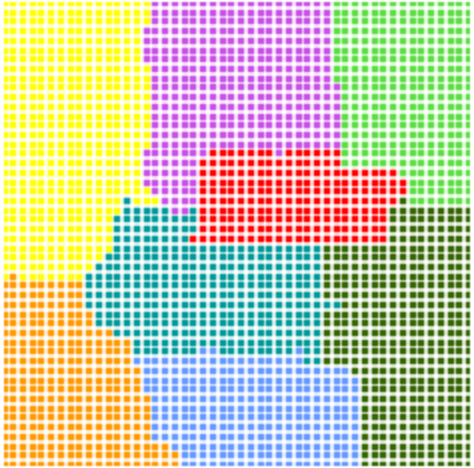
\includegraphics[width=\imgss\textwidth]{images/fields-balacing/2}}
    \caption[short]{krok 2}
\end{subfigure}%

\begin{subfigure}{.5\textwidth}
    \centering
    \fbox{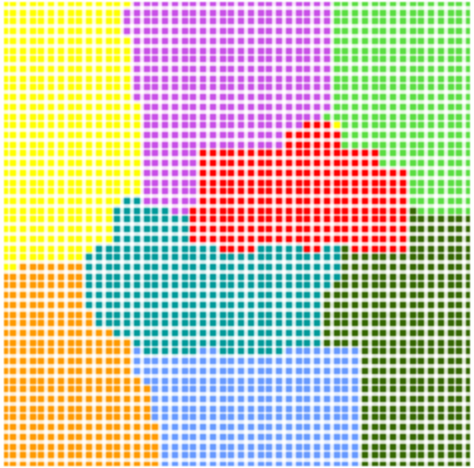
\includegraphics[width=\imgss\textwidth]{images/fields-balacing/3}}
    \caption[short]{krok 3}
\end{subfigure}
\begin{subfigure}{.5\textwidth}
    \centering
    \fbox{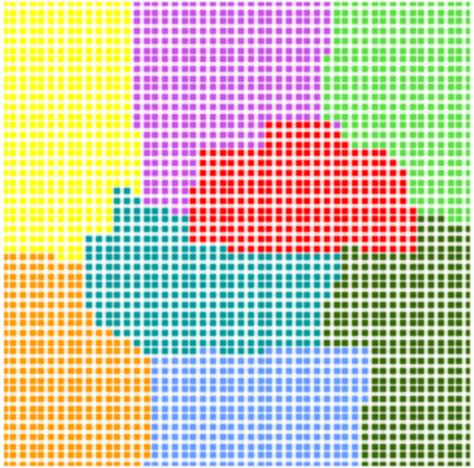
\includegraphics[width=\imgss\textwidth]{images/fields-balacing/4}}
    \caption[short]{krok 4}
\end{subfigure}%

\begin{subfigure}{.5\textwidth}
    \centering
    \fbox{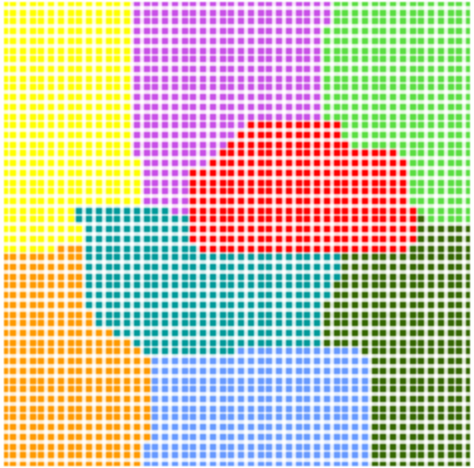
\includegraphics[width=\imgss\textwidth]{images/fields-balacing/5}}
    \caption[short]{krok 5}
\end{subfigure}
\begin{subfigure}{.5\textwidth}
    \centering
    \fbox{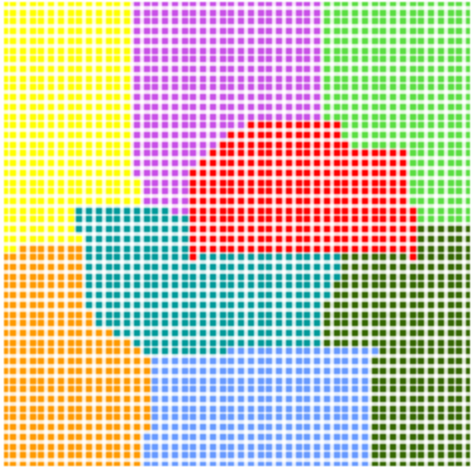
\includegraphics[width=\imgss\textwidth]{images/fields-balacing/6}}
    \caption[short]{krok 6}
\end{subfigure}%
\caption{Obrazki pokazują działania algorytmu optymalizacji granic oraz balansowania rozmiarów pól. Jak widać z wywołania
na wywołanie czerwony obszar, który był na początku najmniejszy, stopniowo rośnie odbierając wierzchołki sąsiednim
obszarom. $p$ wynosi $0.1$.}
\label{im:fields_balancing}
\end{figure}

\newpage
Dla działania algorytmu ustalany jest współczynnik $p$, który decyduje o tym ile wierzchołków zostanie wymienionych.
$p$ osiąga wartości od $0$ do $0.5$ i oznacza jaka część różnicy pól balansowanych obszarów będzie przeniesiona do obszaru
mniejszego.
$V_b$ to wierzchołki wytypowane przez algorytm balansowania pól, które zostaną przeniesione do mniejszego
obszaru.
\begin{equation}
|V_b| = p \cdot ||A| - |B||
\end{equation}

Im $p$ będzie mniejsze tym małe obszary będą rosły wolniej, stopniowo rozbudowując się w kierunku wszystkich sąsiadów.
Im $p$ będzie większe tym proces będzie bardziej gwałtowny, co może bardziej naruszyć podział, na przykład przemieszczając
obszar w jakimś kierunku.
Im $p$ mniejsze, tym więcej wywołań algorytmu optymalizacji potrzebne, aby zrównać wielkość pól obszarów.
Wedle mojego doświadczenia, dla wcześniej użytych współczynników decydujących o częstotliwości
wywołań algorytmu do optymalizacji granic (rysunek \ref{code:main_impr_procedure}), dobrze sprawdza się $p$ wynoszące
około $0.1$, co widać też na rysunku \ref{im:fields_balancing}, gdzie pokazane są wszystkie faktyczne fazy balansowania.
Ze współczynnikiem $0.1$ algorytm miał wystarczająco czasu, aby wyrównać pola.

Dodatkową modyfikacją wprowadzoną przeze mnie był warunek uruchamiania tej części algorytmu, który nie jest obowiązkowy,
ale pełni ważną rolę, kiedy pojawiają się obszary niepodzielne.
Czasami zdarza się, że balansowane obszary ze względu na szczególne ułożenie obszarów niepodzielnych na siatce
mają ze sobą bardzo krótką granicę.
Ta sama sytuacja może pojawić się, gdy rozpatrywany jest klasyczny przypadek bez obszarów
niepodzielnych, ale jest on wtedy znacznie rzadziej spotykany.
W takim przypadku, dodatkowo jeśli $p$ oraz różnica pól balansowanych obszarów jest stosunkowo duża, może dojść
do niekorzystnego balansowania, w którym obszar mniejszy zwiększa swoje pole o dużą liczbę wierzchołków poprzez
stosunkowo krótką granicę.
Aby nie dopuścić do takiego przypadku, stosowany jest prosty warunek, który nie dopuszcza do balansowania
między obszarami, jeśli długość ich granicy przekracza $0.1$ długości dłuższego boku siatki.

